% !TEX root = ../dissertation.tex

\chapter{Computational Geometry}

Computational geometry is defined as the systematic study of algorithms and data structures for geometric objects.
A specific focus is on exact algorithms thar are asymptotically fast.
Computational geometry emerged from the fields of computer science in the late 1970s.
Since that time, the field has grown considerably and has found applications in a large variety of domains, suchs as computer graphics, \gls{gis}, robotics, \gls{CAD}, computer vision, and others.

\section{Mathematical Background}

\section{Incremental Mesh update}

This section we outline our algorithm to incrementally update a mesh. 
Some assumptions:

\begin{itemize}
    \item We first assume that the initial shape model of the asteroid is valid, though not necessarily accurate.
        This means that the mesh is a closed, regular triangular polyhedron.
    \item We assume that there is a sufficient number of vertices in the initial mesh. 
        Therefore during the surface reconstruction phase, the total number of vertices will not vary greatly.
\end{itemize}

The algorithm to insert a point into a given mesh is:

\begin{enumerate}
    \item Determine the distance from the candidate vertex to the mesh.
    \item Identify the closest ``primitive'', i.e. the closest edge, face, or vertex to the candidate point
    \item Incorporate the candidate point into the mesh
\end{enumerate}

There are three possibilities for the closest primitive to the candidate point. 
Based on the distance, there is a different procedure to incorporate the point.

We will demonstrate the methodology of this algorithm with a running example.
Consider the polyhedron shape model of a unit cube centered at the origin.
\begin{figure}
    \centering
    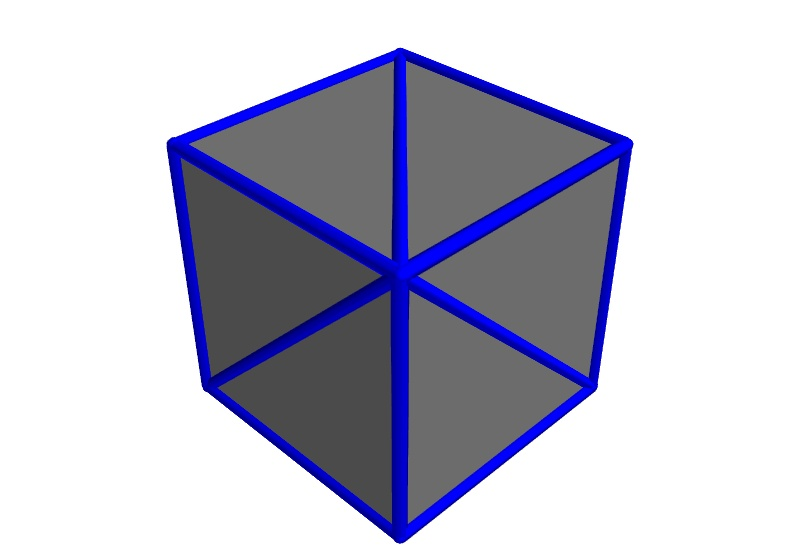
\includegraphics[width=\textwidth]{figures/computational_geometry/cube_mesh.jpg}
    \caption[Polyhedron model of cube]{Long caption~\label{fig:cube_mesh}}
\end{figure}
If the candidate point is closest to a vertex, then you can simply redefine the vertex to be the candidate point.



